\section{How the Command Reviewer Decides}
\label{sec:calibration}
While contextual workflows evaluate proposed writes against workspace code and file snapshots, standalone commands provide only a command string and working directory. We next examine how the command-only branch reconciles ambiguous reference labels and calibrates its operating threshold.
\subsection{When do reviewers have enough evidence?}
The command-only branch must return one of two decisions even when reviewers would prefer to ask for more information. Figure~\ref{fig:label_review} shows where the reference judgments diverged. In the A/B block, A and B gave opposite binary answers on three inputs. On 157 others, one reviewer gave a binary answer and the other chose insufficient evidence. For A/C the corresponding numbers were three and 140, and for B/C they were five and 100. Most disagreement concerned whether the visible evidence sufficed for a decision. Treating every uncertain vote as a hold would conceal that distinction.

\begin{figure}[tb]
\centering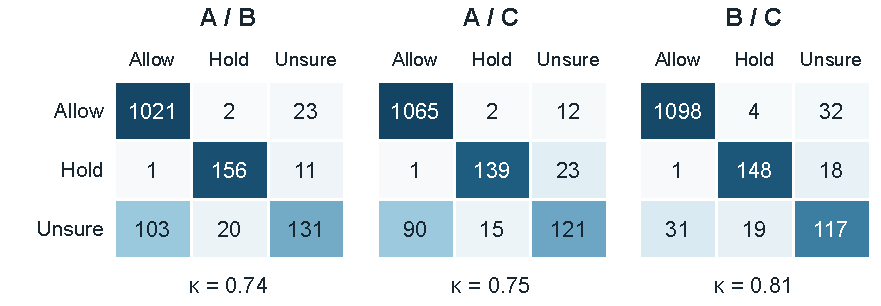
\includegraphics[width=\linewidth]{figures/label_review.pdf}
\caption{Paired judgments before binary scoring. Rows give the first reviewer's judgment and columns the second's. Numbers count unique inputs. Shading shows the fraction within each row. Each block contains 1,468 inputs.}
\Description{Three three-by-three matrices. The largest off-diagonal counts involve an unsure vote, especially for reviewer A.}
\label{fig:label_review}
\end{figure}

Chance-corrected agreement (Cohen's $\kappa$) was .741, .752 and .811 for A/B, A/C and B/C. The pairs received different random blocks. Differences in agreement therefore combine differences among reviewers with differences among commands. The three reviewers also share a model family. Their consensus defines a scoring policy for the evidence supplied, with upstream labels retained where specified in Appendix~\ref{app:external}.

\subsection{Which evidence determines the operating point?}
A lexical score can distinguish commands that name different operations, while an operation profile can associate similar actions across spellings. The two kinds of evidence enter different estimators. For each feature set we estimate a probability of a hold with the lexical model ($p_L$), the randomized trees ($p_T$) and the boosted trees ($p_B$). The selected score and decision rule are
\[
 s = 0.20p_L + 0.65p_T + 0.15p_B,\qquad
 \hat{y}=\mathrm{hold}\ \text{if }s\geq 0.435 .
\]
The numerical threshold applies to this fitted mixture. Its value does not express an estimated probability that a command will cause harm.

\begin{figure}[tb]
\centering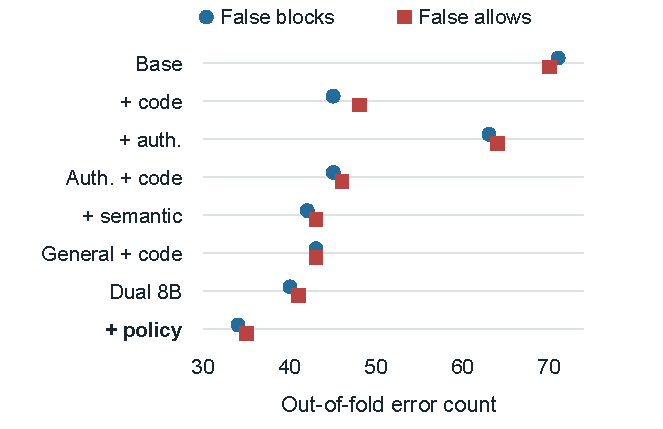
\includegraphics[width=.94\linewidth]{figures/calibration.pdf}
\caption{Five-fold out-of-fold errors for eight feature sets on the 1,750 fitting commands. Each row has its own fitted mixture and threshold. Dots count false blocks and squares count false allows.}
\Description{The baseline has 71 false blocks and 70 false allows. The model using the operations-policy features has 34 and 35.}
\label{fig:calibration}
\end{figure}

Figure~\ref{fig:calibration} explains the choice of features. With static features, the selected operating point yielded 71 false blocks and 70 false allows. Adding code-encoder evidence reduced those counts to 45 and 48. The configuration using both language models and code evidence yielded 40 and 41. Including the policy features reduced the larger error count to 35. Each point incorporates its own threshold and mixture weights. A difference between two rows can result from a change in either the evidence or the calibration. The matched removals in Table~\ref{tab:enc} answer the separate question of what happens when an encoder and its dependent features are removed and the remaining model is refitted.

The three stages produce three distinct error counts. The selected row of Figure~\ref{fig:calibration} has 69 out-of-fold errors. After refitting all three estimators on the 1,750 items, four of those fitting items received the wrong decision. On the 2,653 items with held-out templates, 136 decisions were wrong. Four errors describe the fit to the training rows, 69 describe the scores used for selection, and 136 describe the performance of that selection on other templates.
